% !TEX program = xelatex
\documentclass[UTF8,fontset=fandol,a4paper,11pt]{ctexart}
\usepackage[margin=21mm,top=23mm,bottom=22mm,headheight=16pt]{geometry}
\usepackage{amsmath,amssymb,mathtools,bm}
\usepackage{tikz}
\usetikzlibrary{arrows.meta,calc,angles,quotes,patterns}
\usepackage{xcolor,booktabs,array,longtable,enumitem,fancyhdr,needspace}
\usepackage[unicode,hidelinks]{hyperref}
\definecolor{ink}{HTML}{24343C}
\definecolor{accent}{HTML}{166A70}
\definecolor{muted}{HTML}{65747A}
\definecolor{rulegray}{HTML}{D4DDE0}
\definecolor{warm}{HTML}{966037}
\color{ink}
\setlength{\parindent}{2em}
\setlength{\parskip}{4pt}
\linespread{1.12}
\AtBeginDocument{\setlength{\abovedisplayskip}{6pt plus 2pt minus 1pt}
\setlength{\belowdisplayskip}{6pt plus 2pt minus 1pt}
\setlength{\abovedisplayshortskip}{0pt plus 1pt}
\setlength{\belowdisplayshortskip}{4pt plus 1pt}}
\setlist[enumerate]{label=(\arabic*),leftmargin=2.3em,itemsep=3pt,topsep=4pt}
\setlist[itemize]{leftmargin=2em,itemsep=2pt,topsep=4pt}
\allowdisplaybreaks[1]
\setlength{\emergencystretch}{2em}
\setcounter{secnumdepth}{0}
\providecommand{\tightlist}{\setlength{\itemsep}{0pt}\setlength{\parskip}{0pt}}
\ctexset{section={format=\Large\bfseries\color{accent},beforeskip=10pt,afterskip=9pt},
subsection={format=\normalsize\bfseries\color{accent},beforeskip=10pt,afterskip=4pt},
subsubsection={format=\normalsize\bfseries,beforeskip=8pt,afterskip=3pt}}
\pagestyle{fancy}
\fancyhf{}
\fancyhead[L]{\small\color{muted}物理学难题集萃}
% 页眉仅保留书名；版本名称只在封面显示。
\fancyfoot[L]{\small\color{muted}\chapterlabel}
\fancyfoot[R]{\small\thepage}
\renewcommand{\headrulewidth}{0.4pt}
\renewcommand{\footrulewidth}{0pt}
\newcommand{\dd}{\mathop{}\!\mathrm{d}}
\newcommand{\vect}[1]{\bm{#1}}
\newcommand{\tagline}[1]{\noindent{\small\color{muted}#1}\par}
\newcommand{\result}[1]{\begin{equation*}\boxed{#1}\end{equation*}}
\newcommand{\figcaption}[1]{\par\vspace{2pt}{\small\color{muted}#1}\par}
\newcommand{\teach}[2]{\Needspace{4\baselineskip}\subsection*{讲解要点与追问}#1\par\smallskip\noindent\textbf{追问：}#2\par}
\newcommand{\workarea}{\par\vspace{7mm}\noindent{\small\color{muted}作答区}\par\vspace{4mm}
\noindent\textcolor{rulegray}{\rule{\linewidth}{0.3pt}}\par\vspace{16mm}
\noindent\textcolor{rulegray}{\rule{\linewidth}{0.3pt}}\par\vspace{16mm}
\noindent\textcolor{rulegray}{\rule{\linewidth}{0.3pt}}\par\vspace{16mm}
\noindent\textcolor{rulegray}{\rule{\linewidth}{0.3pt}}}
\tikzset{axis/.style={-{Stealth[length=2mm]},thin,color=muted},
motion/.style={-{Stealth[length=2.3mm]},thick,color=accent},
force/.style={-{Stealth[length=2.3mm]},thick,color=warm},
traj/.style={thick,color=accent},guide/.style={dashed,thin,color=muted},
object/.style={thick,color=ink},every node/.style={font=\small}}\widowpenalty=10000\clubpenalty=10000\displaywidowpenalty=10000\newcommand{\chapterlabel}{光学第二章\quad 光的干涉}







\hypersetup{pdftitle={光学第二章 光的干涉·学生版},pdfauthor={}}

\begin{document}\pdfbookmark[0]{光学第二章 光的干涉}{cover}

\thispagestyle{empty}\vspace*{22mm}

\noindent{\Huge\bfseries 物理学难题集萃}\par\vspace{10mm}

\noindent{\LARGE 光学第二章}\par\vspace{6mm}

\noindent{\LARGE 光的干涉}\par\vspace{12mm}

\noindent{\Large\color{accent}学生版}\par\vspace{9mm}

\noindent\textcolor{accent}{\rule{\linewidth}{1pt}}\par\vspace{9mm}

\noindent 第1--27题\par\vfill\clearpage

\pdfbookmark[1]{题目目录}{contents}\section*{题目目录}

\begin{longtable}{@{}r p{113mm} r@{}}\toprule 题号 & 题目 & 页码\\\midrule

\hyperref[q:1]{1} & \hyperref[q:1]{运动散射体引起的信号起伏} & \pageref{q:1} \\

\hyperref[q:2]{2} & \hyperref[q:2]{射电星升起时的海面干涉} & \pageref{q:2} \\

\hyperref[q:3]{3} & \hyperref[q:3]{菲涅耳双面镜与有限宽光源} & \pageref{q:3} \\

\hyperref[q:4]{4} & \hyperref[q:4]{对剖透镜的条纹数与孔径限制} & \pageref{q:4} \\

\hyperref[q:5]{5} & \hyperref[q:5]{不等间距三缝的主极大与次极大} & \pageref{q:5} \\

\hyperref[q:6]{6} & \hyperref[q:6]{两束斜交平面波的条纹} & \pageref{q:6} \\

\hyperref[q:7]{7} & \hyperref[q:7]{双棱镜的最佳观察距离} & \pageref{q:7} \\

\hyperref[q:8]{8} & \hyperref[q:8]{三平面波的三种组合} & \pageref{q:8} \\

\hyperref[q:9]{9} & \hyperref[q:9]{平面波与球面波的同心环} & \pageref{q:9} \\

\hyperref[q:10]{10} & \hyperref[q:10]{梅斯林装置中的会聚与发散波} & \pageref{q:10} \\

\hyperref[q:11]{11} & \hyperref[q:11]{有限洛埃镜的条纹与谱宽} & \pageref{q:11} \\

\hyperref[q:12]{12} & \hyperref[q:12]{双星角间距的干涉测量} & \pageref{q:12} \\

\hyperref[q:13]{13} & \hyperref[q:13]{均匀狭缝的空间相干性} & \pageref{q:13} \\

\hyperref[q:14]{14} & \hyperref[q:14]{任意扩展光源的可见度公式} & \pageref{q:14} \\

\hyperref[q:15]{15} & \hyperref[q:15]{三块平凸透镜的曲率测量} & \pageref{q:15} \\

\hyperref[q:16]{16} & \hyperref[q:16]{薄膜可见度对角宽和厚度的限制} & \pageref{q:16} \\

\hyperref[q:17]{17} & \hyperref[q:17]{钠双线的条纹可见度拍变} & \pageref{q:17} \\

\hyperref[q:18]{18} & \hyperref[q:18]{圆环收缩中的级次判断} & \pageref{q:18} \\

\hyperref[q:19]{19} & \hyperref[q:19]{光电条纹信号与双线拍频} & \pageref{q:19} \\

\hyperref[q:20]{20} & \hyperref[q:20]{法布里—珀罗双线的分数级次} & \pageref{q:20} \\

\hyperref[q:21]{21} & \hyperref[q:21]{多光束条纹的半强度宽} & \pageref{q:21} \\

\hyperref[q:22]{22} & \hyperref[q:22]{谐振腔的模间隔与腔峰宽度} & \pageref{q:22} \\

\hyperref[q:23]{23} & \hyperref[q:23]{平行玻璃膜的反射与透射反衬度} & \pageref{q:23} \\

\hyperref[q:24]{24} & \hyperref[q:24]{单层减反膜的厚度与波长响应} & \pageref{q:24} \\

\hyperref[q:25]{25} & \hyperref[q:25]{半球发光器件的增透设计} & \pageref{q:25} \\

\hyperref[q:26]{26} & \hyperref[q:26]{单层多光束求和与双层减反} & \pageref{q:26} \\

\hyperref[q:27]{27} & \hyperref[q:27]{交替四分之一波层的高反射膜} & \pageref{q:27} \\

\bottomrule\end{longtable}

\clearpage

\pdfbookmark[2]{第 1 题 运动散射体引起的信号起伏}{q1}

\section*{第 1 题\quad 运动散射体引起的信号起伏}\label{q:1}

汽车沿东西向公路由东向西匀速行驶。公路南侧的接收机$H$接收从西南远处传来的$f=60\,\mathrm{MHz}$电磁波，汽车将同一信号散射到$H$。$H$到公路的垂距为$L=100\,\mathrm m$。汽车到达$H$正北方时，信号强度起伏频率为$2\,\mathrm{Hz}$；汽车继续向西行驶$200\,\mathrm m$时，起伏频率降为零。求电磁波的传播方位和车速。忽略传播时延对汽车位置的修正。

\begin{center}\begin{minipage}{.98\linewidth}\centering
\begin{tikzpicture}[scale=.85,transform shape]
\draw[object] (-5.50000,0.00000)--(2.00000,0.00000);\fill (0.00000,0.00000) circle(.035);\node[above right] at (0.00000,0.00000) {$C$};\fill (0.00000,-2.00000) circle(.035);\node[below] at (0.00000,-2.00000) {$H$};\draw[guide] (0.00000,0.00000)--(0.00000,-2.00000);\draw[<->,thin,color=muted] (0.70000,0.00000)--(0.70000,-2.00000);\node[right] at (0.70000,-1.00000) {$L$};\fill (-4.00000,0.00000) circle(.035);\node[above] at (-4.00000,0.00000) {$B$};\draw[motion] (-3.30000,0.50000)--(-4.40000,0.50000);\node[above] at (-3.80000,0.50000) {$v$};\draw[motion] (-6.00000,-1.00000)--(-4.00000,0.00000);\draw[motion] (-2.00000,-3.00000)--(0.00000,-2.00000);\draw[motion] (-4.00000,0.00000)--(0.00000,-2.00000);\node[below] at (-5.50000,-0.70000) {来波};\draw[<->,thin,color=muted] (-4.00000,-0.35000)--(0.00000,-0.35000);\node[below] at (-2.00000,-0.35000) {$200\,\mathrm m$};
\end{tikzpicture}
\figcaption{图光2.1\quad 道路、接收机与汽车的位置}
\end{minipage}\end{center}

\workarea

\clearpage

\pdfbookmark[2]{第 2 题 射电星升起时的海面干涉}{q2}

\section*{第 2 题\quad 射电星升起时的海面干涉}\label{q:2}

接收天线距平静海面$h=2.00\,\mathrm m$，记录电场垂直于竖直入射面的水平分量。一颗射电星发出$\lambda=21.0\,\mathrm{cm}$的电磁波，逐渐从海平面升起。把海水近似为实折射率$n>1$、无吸收的介质，空气折射率为1。（1）求各级干涉极大、极小的仰角。（2）说明刚升起时强度怎样变化。（3）给出相邻极大、极小的强度表达式，并讨论菲涅耳反射系数随角度变化所带来的限制。

\begin{center}\begin{minipage}{.98\linewidth}\centering
\begin{tikzpicture}[font=\small,scale=.85,transform shape]
\draw[object] (-5.7,0)--(1.7,0);\node[below]at(1.15,0){海面};
\fill(0,1.6)circle(1.4pt);\node[right]at(0,1.6){$A$};
\fill(-4,0)circle(1.4pt);\node[below left]at(-4,0){$B$};
\draw[motion](-5.3,.52)--(-4,0);\draw[motion](-4,0)--(0,1.6);
\draw[motion](-5,3.6)--(0,1.6);
\draw[guide](-4,0)--(-2.6,0);
\draw[thin](-3.2,0)arc(0:21.8014:.8);\node[above]at(-2.95,.15){$\theta$};
\draw[<->,thin](.65,0)--(.65,1.6);\node[right]at(.65,.8){$h$};
\node[above]at(-3.3,3.1){平行来波};\end{tikzpicture}
\figcaption{图光2.2\quad 海面反射与直达接收的几何关系}
\end{minipage}\end{center}

\workarea

\clearpage

\pdfbookmark[2]{第 3 题 菲涅耳双面镜与有限宽光源}{q3}

\section*{第 3 题\quad 菲涅耳双面镜与有限宽光源}\label{q:3}

菲涅耳双面镜的两镜夹小角$\alpha=20'$，狭缝光源距两镜交线$R=10\,\mathrm{cm}$。波长$\lambda=600\,\mathrm{nm}$，屏与两虚光源的连线平行，屏距镜交线$L=210\,\mathrm{cm}$。狭缝位于对称位置，镜面足够大。（1）求条纹间距、重叠区宽度和其中亮纹条数。（2）$R$增大为两倍时怎样变化？（3）光源沿横向移动$\delta s$时条纹怎样移动？（4）均匀非相干狭缝的宽度多大时条纹第一次消失？采用小角近似，并说明计数口径。

\begin{center}\begin{minipage}{.97\linewidth}\centering
\begin{tikzpicture}[x=.003cm,y=.07cm,font=\small]
\fill[accent!6] (0,0)--(2100,12.2174426)--(2100,-12.2174426)--cycle;
\draw[axis] (-360,0)--(2300,0) node[right]{$x/\mathrm{mm}$};
\draw[object] (2100,-16)--(2100,16);
\draw[guide] (-99.9983077,.5817731)--(0,0);
\draw[guide] (-99.9983077,-.5817731)--(0,0);
\draw[motion] (0,0)--(2100,-12.2174426);
\draw[force] (0,0)--(2100,12.2174426);
\fill (-99.9983077,.5817731) circle[radius=.55pt];
\fill (-99.9983077,-.5817731) circle[radius=.55pt];
\draw[thin,color=muted] (-99.9983077,.5817731)--(-220,5);
\draw[thin,color=muted] (-99.9983077,-.5817731)--(-220,-5);
\node[left] at(-220,5){$S_1$};\node[left] at(-220,-5){$S_2$};
\fill (0,0) circle[radius=1pt];\node[below right] at(0,-1){$O$};
\node[above right] at(2100,12.2174426){$M$};
\node[below right] at(2100,-12.2174426){$N$};
\node[above] at(2100,16){屏};
\draw[<->,thin,color=muted] (0,-19)--(2100,-19) node[midway,below]{$L=2100\,\mathrm{mm}$};
\node[below,align=center] at(1050,-27){横纵异比例；两虚光源的坐标为\\$(-R\cos\alpha,\ \pm R\sin\alpha)$。};
\end{tikzpicture}
\figcaption{图光2.3\quad 两镜交线限定照明边界，虚光源提供相位基准}
\end{minipage}\end{center}

\workarea

\clearpage

\pdfbookmark[2]{第 4 题 对剖透镜的条纹数与孔径限制}{q4}

\section*{第 4 题\quad 对剖透镜的条纹数与孔径限制}\label{q:4}

将焦距$f=10\,\mathrm{cm}$的薄会聚透镜沿直径剖成两半，沿垂直于切口方向把两半的光心间距拉开到$\delta=1.0\,\mathrm{mm}$。单色点光源位于两半光心中点的轴上，距透镜$s=20\,\mathrm{cm}$；波长$\lambda=500\,\mathrm{nm}$。屏位于透镜后$L=50\,\mathrm{cm}$。求条纹间距、共同照明宽度和亮纹条数，并说明有限透镜孔径何时改变结果。

\begin{center}\begin{minipage}{.98\linewidth}\centering
\begin{tikzpicture}[scale=.8,transform shape]
\draw[axis] (-3.70000,0.00000)--(8.00000,0.00000);\fill (-3.00000,0.00000) circle(.035);\node[below] at (-3.00000,0.00000) {$Q$};\draw[object] (0.00000,0.20000)--(0.00000,1.40000);\draw[object] (0.00000,-0.20000)--(0.00000,-1.40000);\fill (0.00000,0.20000) circle(.035);\node[above left] at (0.00000,0.20000) {$O_1$};\fill (0.00000,-0.20000) circle(.035);\node[below left] at (0.00000,-0.20000) {$O_2$};\draw[object] (7.50000,-1.90000)--(7.50000,1.90000);\node[above] at (7.50000,1.90000) {屏};\draw[<->,thin,color=muted] (-3.00000,-1.80000)--(0.00000,-1.80000);\node[below] at (-1.50000,-1.80000) {$s$};\draw[<->,thin,color=muted] (0.00000,-1.80000)--(7.50000,-1.80000);\node[below] at (3.75000,-1.80000) {$L$};\draw[motion] (-3.00000,0.00000)--(0.00000,0.20000);
\draw[motion] (0.00000,0.20000)--(7.50000,0.70000);\draw[motion] (-3.00000,0.00000)--(0.00000,-0.20000);
\draw[motion] (0.00000,-0.20000)--(7.50000,-0.70000);\draw[motion] (-3.00000,0.00000)--(0.00000,1.40000);
\draw[motion] (0.00000,1.40000)--(3.00000,0.40000);
\draw[motion] (3.00000,0.40000)--(7.50000,-1.10000);\draw[motion] (-3.00000,0.00000)--(0.00000,-1.40000);
\draw[motion] (0.00000,-1.40000)--(3.00000,-0.40000);
\draw[motion] (3.00000,-0.40000)--(7.50000,1.10000);\fill (3.00000,0.40000) circle(.035);\node[above] at (3.00000,0.40000) {$Q_1$};\fill (3.00000,-0.40000) circle(.035);\node[below] at (3.00000,-0.40000) {$Q_2$};
\end{tikzpicture}
\figcaption{图光2.4\quad 两半透镜的像点与内外边缘光线}
\end{minipage}\end{center}

图中纵横比例不同；横向放大以显示毫米量级的像点间距和切口。图示边界取半片有效高度$a=3\,\mathrm{mm}$作为孔径检验的一个例子。

\workarea

\clearpage

\pdfbookmark[2]{第 5 题 不等间距三缝的主极大与次极大}{q5}

\section*{第 5 题\quad 不等间距三缝的主极大与次极大}\label{q:5}

三个平行窄缝沿竖直方向排列，相邻间距依次为$d$和$3d/2$。三缝等宽，缝宽远小于$\lambda$，受同相单色光照明；远屏上观察方向与轴夹小角$\theta$，各缝单独产生的强度均近似为$I_s$。（1）求强度分布。（2）求零级以外首个完全相长的主极大，并说明它与最近局部极大的区别。（3）求主极大角位置一半处与主极大的强度比。

\begin{center}\begin{minipage}{.98\linewidth}\centering
\begin{tikzpicture}[font=\small,scale=.85,transform shape]
\draw[object](0,.4)--(0,-2.9);
\fill(0,0)circle(1.5pt);\node[left]at(0,0){$S_1$};
\fill(0,-1)circle(1.5pt);\node[left]at(0,-1){$S_2$};
\fill(0,-2.5)circle(1.5pt);\node[left]at(0,-2.5){$S_3$};
\draw[motion](0,0)--(6,1.2);\draw[motion](0,-1)--(6,.2);\draw[motion](0,-2.5)--(6,-1.3);
\draw[guide](0,0)--(3,0);\draw[thin](2.4,0)arc(0:11.30993247:2.4);\node at(2.8,.28){$\theta$};
\draw[<->,thin](-.75,0)--(-.75,-1);\node[left]at(-.75,-.5){$d$};
\draw[<->,thin](-.75,-1)--(-.75,-2.5);\node[left]at(-.75,-1.75){$3d/2$};
\node[above]at(4,1.4){远场同一观察方向};
\node[anchor=north]at(2.5,-3.2){沿缝间连线的坐标：$0,d,5d/2$。};
\end{tikzpicture}
\figcaption{图光2.5\quad 三缝坐标及远场方向的平行光线}
\end{minipage}\end{center}

\workarea

\clearpage

\pdfbookmark[2]{第 6 题 两束斜交平面波的条纹}{q6}

\section*{第 6 题\quad 两束斜交平面波的条纹}\label{q:6}

两束同频、同偏振相干平面光波的波长均为$\lambda$，振幅之比为$2:1$，传播方向夹角为$\theta$。观察屏垂直于两传播方向的角平分线。求条纹的反衬度、方向与间距；说明夹角趋近零的极限。

当两传播方向不平行时，共同线偏振方向取为垂直于两波矢所在平面。图中用$\odot$标明这一电场方向，传播箭头旁的$2A,A$只表示振幅。

\begin{center}\begin{minipage}{.97\linewidth}\centering
\begin{tikzpicture}
\begin{scope}[x=1.2cm,y=1.2cm]
\draw[axis](-2.7,0)--(3.2,0)node[right]{$z$};
\draw[object](0,-1.8)--(0,2.0)node[above]{$x$};
\draw[motion](-2.25166605,1.3)--(2.25166605,-1.3)node[below right]{$\boldsymbol k_1$};
\draw[force](-2.25166605,-1.3)--(2.25166605,1.3)node[above right]{$\boldsymbol k_2$};
\fill(0,0)circle[radius=1pt];\node[above]at(-1,.04){$O$};\draw[thin,color=muted](-.85,.08)--(0,0);
\draw[thin](.73612159,-.425)arc[start angle=-30,end angle=30,radius=.85];
\node[above right]at(.84,.04){$\theta$};
\node[above]at(-1.8,1.55){振幅$2A$};
\node[below]at(-1.8,-1.55){振幅$A$};
\node[right]at(.25,1.8){屏$z=0$};
\node[align=center]at(.1,-2.55){两束共同偏振：$\odot\,{+y}$\\几何取$\theta=60^\circ$作图};
\end{scope}
\end{tikzpicture}
\figcaption{图光2.6\quad 箭头表示传播方向；共同电场方向垂直于$xz$平面}
\end{minipage}\end{center}

\workarea

\clearpage

\pdfbookmark[2]{第 7 题 双棱镜的最佳观察距离}{q7}

\section*{第 7 题\quad 双棱镜的最佳观察距离}\label{q:7}

波长$\lambda=632.8\,\mathrm{nm}$的平行光垂直照到菲涅耳双棱镜上。每个半棱镜的折射顶角为$\alpha=3'30''$，总通光宽度$W=4.0\,\mathrm{cm}$，折射率$n=1.5$。求屏距$L$为何值时共同照明区及条纹数最大，何时共同照明区消失，并计算最大条纹覆盖数和对称区内实际亮纹条数。两半等厚、同相，忽略边缘衍射。

\begin{center}\begin{minipage}{.98\linewidth}\centering
\begin{tikzpicture}[x=0.160000000cm,y=.12cm]
\draw[axis](-4.000000000000,0.000000000000)--(43.860045903905,0.000000000000)node[right]{$z/\mathrm m$};
\draw[object](0.000000000000,-20.000000000000)--(0.000000000000,20.000000000000);
\draw[motion](-3.000000000000,20.000000000000)--(0.000000000000,20.000000000000);
\draw[motion](-3.000000000000,0.000000000000)--(0.000000000000,0.000000000000);
\draw[motion](-3.000000000000,-20.000000000000)--(0.000000000000,-20.000000000000);
\draw[motion](0.000000000000,20.000000000000)--(40.860045903905,-0.800000000000);
\draw[motion](0.000000000000,0.000000000000)--(40.860045903905,-20.800000000000);
\draw[force](0.000000000000,0.000000000000)--(40.860045903905,20.800000000000);
\draw[force](0.000000000000,-20.000000000000)--(40.860045903905,0.800000000000);
\draw[object](19.644252838416,-24.000000000000)--(19.644252838416,24.000000000000);
\node[above]at(19.644252838416,24.000000000000){屏};
\node[below]at(0.000000000000,-24.000000000000){偏折等效面};
\node[above,align=center]at(-3.200000000000,24.000000000000){$y/\mathrm{mm}$\\横向放大};
\draw[guide](39.288505676831,-24.000000000000)--(39.288505676831,24.000000000000);
\node[above]at(39.288505676831,24.000000000000){$L_0$};
\node[below right]at(19.644252838416,-24.000000000000){$L_*$};
\node[below right]at(39.288505676831,-24.000000000000){$39.2885\,\mathrm m$};
\node[below left]at(-2.000000000000,20.000000000000){$20$};
\node[above left]at(-2.000000000000,-20.000000000000){$-20$};
\end{tikzpicture}
\figcaption{图光2.7\quad 两束的四条边界；轴向米、横向毫米}
\end{minipage}\end{center}

图用零厚度棱镜等效面表示偏折；横向放大，$z$用米、$y$用毫米。请区分连续覆盖数最大时的屏距和整数亮纹数达到最大值的屏距范围。

\workarea

\clearpage

\pdfbookmark[2]{第 8 题 三平面波的三种组合}{q8}

\section*{第 8 题\quad 三平面波的三种组合}\label{q:8}

三束同频、同偏振平面波在$xz$平面内传播，波长均为$\lambda$，波矢$\boldsymbol k_2$沿$+z$，$\boldsymbol k_1,\boldsymbol k_3$分别与$+z$成$\pm\theta$。振幅依次为$A_0,2A_0,A_0$，在原点的相位相同。屏为$z=0$。分别求三束同时存在、仅保留第1与3束、仅保留第1与2束时的强度分布、反衬度和条纹间距，并比较图样。

\begin{center}\begin{minipage}{.98\linewidth}\centering
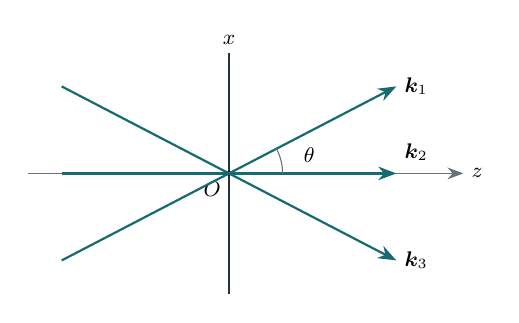
\begin{tikzpicture}[scale=.85,transform shape]
\draw[axis] (-3.00000,0.00000)--(3.50000,0.00000);\draw[object] (0.00000,-1.80000)--(0.00000,1.80000);\fill (0.00000,0.00000) circle(.035);\node[below left] at (0.00000,0.00000) {$O$};\node[above] at (0.00000,1.80000) {$x$};\node[right] at (3.50000,0.00000) {$z$};\draw[motion] (-2.50000,-1.30000)--(2.50000,1.30000);\node[right] at (2.50000,1.30000) {$\boldsymbol k_1$};\draw[motion] (-2.50000,0.00000)--(2.50000,0.00000);\node[above right,yshift=2pt] at (2.50000,0.00000) {$\boldsymbol k_2$};\draw[motion] (-2.50000,1.30000)--(2.50000,-1.30000);\node[right] at (2.50000,-1.30000) {$\boldsymbol k_3$};\draw[thin,color=muted] (.8,0) arc[start angle=0,end angle=27.47443,radius=.8];\node[] at (1.20000,0.28000) {$\theta$};
\end{tikzpicture}
\figcaption{图光2.8\quad 传播平面与$z=0$接收屏}
\end{minipage}\end{center}

取$A_0>0$，$0<\theta<\pi/2$；共同线偏振沿$y$方向，垂直于传播平面。强度按同一比例常数乘以合振幅模平方定义。图中屏为$x$轴所在的$z=0$平面截线。

\workarea

\clearpage

\pdfbookmark[2]{第 9 题 平面波与球面波的同心环}{q9}

\section*{第 9 题\quad 平面波与球面波的同心环}\label{q:9}

振幅为$A$、波数为$k=2\pi/\lambda$的平面波沿$+z$传播；原点$O$的同频点源发出球面波。球面波在距$O$一个单位长度处的振幅为平面波振幅的$D$倍，其中$D$按同一长度单位取数值；两波在轴上的参考相位相同。屏位于$z=D$，屏中心强度为$I_c$。求屏上近轴区的强度分布和条纹形状、半径及间距，并说明振幅和相位近似的区别。

\begin{center}\begin{minipage}{.98\linewidth}\centering
\begin{tikzpicture}[x=1.3cm,y=1.3cm]
\draw[axis](-.5,0)--(5,0)node[right]{$z$};
\draw[object](4,-1.8)--(4,2)node[above]{屏};
\fill(0,0)circle(.035);\node[below left]at(0,0){$O$};
\node[below right]at(4,0){$C$};
\draw[color=warm,thin]plot coordinates {(0.877582561890,-0.479425538604) (0.889292721623,-0.457338447179) (0.900447102353,-0.434965534111) (0.911038732954,-0.412320781743) (0.921060994003,-0.389418342309) (0.930507621912,-0.366272529086) (0.939372712847,-0.342897807455) (0.947650726415,-0.319308785857) (0.955336489126,-0.295520206661) (0.962425197628,-0.271546936956) (0.968912421711,-0.247403959255) (0.974794107069,-0.223106362132) (0.980066577841,-0.198669330795) (0.984726538905,-0.174108137594) (0.988771077936,-0.149438132474) (0.992197667229,-0.124674733385) (0.995004165278,-0.099833416647) (0.997188818112,-0.074929707273) (0.998750260395,-0.049979169271) (0.999687516276,-0.024997395915) (1.000000000000,0.000000000000) (0.999687516276,0.024997395915) (0.998750260395,0.049979169271) (0.997188818112,0.074929707273) (0.995004165278,0.099833416647) (0.992197667229,0.124674733385) (0.988771077936,0.149438132474) (0.984726538905,0.174108137594) (0.980066577841,0.198669330795) (0.974794107069,0.223106362132) (0.968912421711,0.247403959255) (0.962425197628,0.271546936956) (0.955336489126,0.295520206661) (0.947650726415,0.319308785857) (0.939372712847,0.342897807455) (0.930507621912,0.366272529086) (0.921060994003,0.389418342309) (0.911038732954,0.412320781743) (0.900447102353,0.434965534111) (0.889292721623,0.457338447179) (0.877582561890,0.479425538604)};
\draw[color=warm,thin]plot coordinates {(1.755165123781,-0.958851077208) (1.778585443246,-0.914676894358) (1.800894204705,-0.869931068222) (1.822077465908,-0.824641563487) (1.842121988006,-0.778836684617) (1.861015243825,-0.732545058172) (1.878745425695,-0.685795614911) (1.895301452830,-0.638617571714) (1.910672978251,-0.591040413323) (1.924850395256,-0.543093873912) (1.937824843421,-0.494807918509) (1.949588214138,-0.446212724263) (1.960133155682,-0.397338661590) (1.969453077810,-0.348216275187) (1.977542155872,-0.298876264947) (1.984395334459,-0.249349466770) (1.990008330556,-0.199666833294) (1.994377636224,-0.149859414545) (1.997500520790,-0.099958338541) (1.999375032551,-0.049994791829) (2.000000000000,0.000000000000) (1.999375032551,0.049994791829) (1.997500520790,0.099958338541) (1.994377636224,0.149859414545) (1.990008330556,0.199666833294) (1.984395334459,0.249349466770) (1.977542155872,0.298876264947) (1.969453077810,0.348216275187) (1.960133155682,0.397338661590) (1.949588214138,0.446212724263) (1.937824843421,0.494807918509) (1.924850395256,0.543093873912) (1.910672978251,0.591040413323) (1.895301452830,0.638617571714) (1.878745425695,0.685795614911) (1.861015243825,0.732545058172) (1.842121988006,0.778836684617) (1.822077465908,0.824641563487) (1.800894204705,0.869931068222) (1.778585443246,0.914676894358) (1.755165123781,0.958851077208)};
\draw[color=warm,thin]plot coordinates {(2.632747685671,-1.438276615813) (2.667878164870,-1.372015341537) (2.701341307058,-1.304896602334) (2.733116198862,-1.236962345230) (2.763182982009,-1.168255026926) (2.791522865737,-1.098817587258) (2.818118138542,-1.028693422366) (2.842952179244,-0.957926357571) (2.866009467377,-0.886560619984) (2.887275592885,-0.814640810868) (2.906737265132,-0.742211877764) (2.924382321207,-0.669319086395) (2.940199733524,-0.596007992385) (2.954179616715,-0.522324412781) (2.966313233808,-0.448314397421) (2.976593001688,-0.374024200156) (2.985012495834,-0.299500249940) (2.991566454337,-0.224789121818) (2.996250781185,-0.149937507812) (2.999062548827,-0.074992187744) (3.000000000000,0.000000000000) (2.999062548827,0.074992187744) (2.996250781185,0.149937507812) (2.991566454337,0.224789121818) (2.985012495834,0.299500249940) (2.976593001688,0.374024200156) (2.966313233808,0.448314397421) (2.954179616715,0.522324412781) (2.940199733524,0.596007992385) (2.924382321207,0.669319086395) (2.906737265132,0.742211877764) (2.887275592885,0.814640810868) (2.866009467377,0.886560619984) (2.842952179244,0.957926357571) (2.818118138542,1.028693422366) (2.791522865737,1.098817587258) (2.763182982009,1.168255026926) (2.733116198862,1.236962345230) (2.701341307058,1.304896602334) (2.667878164870,1.372015341537) (2.632747685671,1.438276615813)};
\draw[guide](0.700000000000,-1.600000000000)--(0.700000000000,1.650000000000);
\draw[guide](1.700000000000,-1.600000000000)--(1.700000000000,1.650000000000);
\draw[guide](2.700000000000,-1.600000000000)--(2.700000000000,1.650000000000);
\draw[force](0.000000000000,0.000000000000)--(4.000000000000,1.500000000000);
\draw[motion](-0.300000000000,1.500000000000)--(4.000000000000,1.500000000000);
\draw[motion](-0.300000000000,-1.100000000000)--(4.000000000000,-1.100000000000);
\fill(4,1.5)circle(.035);\node[right]at(4,1.5){$P$};
\draw[<->,thin,color=muted](4.6,0)--(4.6,1.5);\node[right]at(4.6,.75){$\rho$};
\draw[<->,thin,color=muted](0,-2)--(4,-2);\node[below]at(2,-2){$D$};
\node[above]at(1.1,2.15){平面波：虚线波前};\node[below]at(2,-2.65){球面波：以$O$为中心的弧线波前};
\end{tikzpicture}
\figcaption{图光2.9\quad 同轴平面波与球面波在屏上重叠}
\end{minipage}\end{center}

\workarea

\clearpage

\pdfbookmark[2]{第 10 题 梅斯林装置中的会聚与发散波}{q10}

\section*{第 10 题\quad 梅斯林装置中的会聚与发散波}\label{q:10}

把同一薄会聚透镜沿直径剖开，两半沿主轴错开$8.0\,\mathrm{cm}$。点光源$S$在轴上，距较近半透镜$L_1$为$60\,\mathrm{cm}$；两半焦距均$f=30\,\mathrm{cm}$。两半分别成像于$S_1',S_2'$，在两像点中间、垂直轴放屏，波长为$500\,\mathrm{nm}$。（1）求近轴干涉条纹的形状。（2）给出相邻环的半径平方差；若中心调为亮纹，求各级亮环半径及间距。保留可能存在的常相位差。



\Needspace{6\baselineskip}

\begin{center}\begin{minipage}{.98\linewidth}\centering
\begin{tikzpicture}[font=\small,x=.05cm,y=.8cm]
\draw[axis](-5,0)--(137,0);\node[right]at(137,0){$z$};
\fill(0,0)circle(1.5pt);\node[below]at(0,0){$S$};
\draw[object](60,0)--(60,1.2);\draw[object](68,0)--(68,-1.2);
\node[above]at(60,1.2){$L_1$};\node[below]at(68,-1.2){$L_2$};
\draw[motion](0,0)--(60,1);\draw[motion](60,1)--(120,0);
\draw[motion](120,0)--(132,-.2);
\draw[motion](0,0)--(68,-1);\draw[motion](68,-1)--(121.6842105263,0);
\fill(120,0)circle(1.2pt);\fill(121.6842105263,0)circle(1.2pt);
\draw[object](120.8421052632,-1.5)--(120.8421052632,1.5);\node[above]at(120.8421052632,1.5){屏};
\draw[guide](120,0)--(109,-.9);\node[below]at(109,-.9){$S_1'$};
\draw[guide](121.6842105263,0)--(133,.65);\node[above]at(133,.65){$S_2'$};
\draw[<->,thin](0,-1.8)--(60,-1.8);\node[below]at(30,-1.8){$60\,\mathrm{cm}$};
\draw[<->,thin](60,1.9)--(68,1.9);\node[above]at(64,1.9){$8\,\mathrm{cm}$};
\node[anchor=north,align=center]at(65,-2.55){轴向从$S$量起：$120$与$121.68421\,\mathrm{cm}$。\\横纵异比例；图示光线不限定半片口径。};
\end{tikzpicture}
\figcaption{图光2.10\quad 两半透镜的像点与夹在其间的屏}
\end{minipage}\end{center}

\workarea

\clearpage

\pdfbookmark[2]{第 11 题 有限洛埃镜的条纹与谱宽}{q11}

\section*{第 11 题\quad 有限洛埃镜的条纹与谱宽}\label{q:11}

水平洛埃镜长度$B=5.00\,\mathrm{cm}$，镜左端$x=0$、右端$x=B$，屏在$x=B+C$，其中$C=5.00\,\mathrm m$。点光源在$(-A,d)$，$A=2.00\,\mathrm{cm}$、$d=0.500\,\mathrm{mm}$，波长$\lambda=600\,\mathrm{nm}$，反射附加相位为$\pi$。（1）求近轴条纹间距。（2）求共同照明高度范围和实际亮纹数。（3）为在全部共同区内保持可辨条纹，对光谱宽度有何要求？给出所采用的可见度判据。

\begin{center}\begin{minipage}{.98\linewidth}\centering
\begin{tikzpicture}
\begin{scope}[x=.52cm,y=.85cm]
\draw[axis] (-2.8,0)--(9.2,0) node[right] {$x/\mathrm{cm}$};
\draw[axis] (0,-.75)--(0,2.45) node[above] {$y/\mathrm{mm}$};
\draw[very thick] (0,0)--(5,0);
\fill (-2,.5) circle(1.3pt) node[above left] {$S$};
\fill (-2,-.5) circle(1.3pt) node[below left] {$S'$};
\draw[motion] (-2,.5)--(0,0);
\draw[motion] (0,0)--(8,2) node[above right] {至$H_2$};
\draw[force] (-2,.5)--(5,0);
\draw[force] (5,0)--(8,.214286);
\node[above] at (7.8,.45) {至$H_1$};
\draw[guide] (-2,-.5)--(0,0);
\draw[guide] (-2,-.5)--(5,0);
\draw[muted] (5,0)--(5,-.08) node[below] {$5$};
\node[left] at (0,1.2) {$x=0$};
\draw[muted] (-2,0)--(-2,-.08) node[below left] {$-2$};
\end{scope}
\begin{scope}[shift={(7.5cm,0)},x=1cm,y=.025cm]
\draw[axis] (0,0)--(0,145) node[above] {$y/\mathrm{mm}$};
\fill[accent,opacity=.12] (-.12,35.714286) rectangle (.12,126.25);
\draw[object] (0,35.714286)--(0,126.25);
\draw[accent,fill=white] (0,35.714286) circle(1.4pt);
\draw[accent,fill=white] (0,126.25) circle(1.4pt);
\draw[muted] (-.12,35.714286)--(.12,35.714286);
\draw[muted] (-.12,126.25)--(.12,126.25);
\node[right,align=left] at (.18,35.714286) {$H_1$\\$35.7143$};
\node[right,align=left] at (.18,126.25) {$H_2$\\$126.250$};
\node[below,align=center] at (.5,-8) {屏截线\\$x=5.05\,\mathrm m$};
\end{scope}
\end{tikzpicture}
\figcaption{图光2.11\quad 左：镜旁局部；右：屏上共同照明区}
\end{minipage}\end{center}

镜面两端作为共同区边界，不纳入计数；忽略衍射与遮挡，两路取共同的垂直纸面线偏振，光源和虚像保持相干。讨论谱宽时先采用等幅两束、反射相位在窄带内恒为$\pi$的理想模型，再说明谱形和阈值。图左的坐标单位为厘米和毫米，两条边缘出射线继续传播到右图屏上的$H_2,H_1$。

\workarea

\clearpage

\pdfbookmark[2]{第 12 题 双星角间距的干涉测量}{q12}

\section*{第 12 题\quad 双星角间距的干涉测量}\label{q:12}

间距可调为$d$的两小孔后放会聚透镜，在后焦面观察遥远双星的干涉条纹。双星可近似为等亮、彼此非相干的点源，沿两孔连线的角间距为$\theta$，装置对准角平分线。两孔距从小连续增大时，条纹反衬度周期变化；平均波长$\lambda=550\,\mathrm{nm}$，在$d=2.0\,\mathrm{mm}$时第一次消失。解释现象并求$\theta$；若双星不等亮，现象怎样改变？

\begin{center}\begin{minipage}{.98\linewidth}\centering
\begin{tikzpicture}[scale=.85,transform shape]
\draw[object] (0.00000,-1.60000)--(0.00000,1.60000);\fill (0.00000,0.60000) circle(.035);\node[above left,xshift=-4pt,yshift=7pt,fill=white,inner sep=1pt] at (0.00000,0.60000) {$S_1$};\fill (0.00000,-0.60000) circle(.035);\node[below left,xshift=-4pt,yshift=-7pt,fill=white,inner sep=1pt] at (0.00000,-0.60000) {$S_2$};\draw[object] (0.80000,-1.50000)--(0.80000,1.50000);\draw[object] (0.67000,-1.30000)--(0.80000,-1.50000)--(0.93000,-1.30000);\draw[object] (0.67000,1.30000)--(0.80000,1.50000)--(0.93000,1.30000);\node[above] at (0.80000,1.60000) {$L$};\draw[object] (6.00000,-1.70000)--(6.00000,1.70000);\node[above] at (6.00000,1.70000) {焦面};\draw[motion] (-3.00000,1.40000)--(0.00000,0.60000);\draw[motion] (-3.00000,0.20000)--(0.00000,-0.60000);\draw[force] (-3.00000,-1.40000)--(0.00000,-0.60000);\draw[force] (-3.00000,-0.20000)--(0.00000,0.60000);\draw[<->,thin,color=muted] (-0.50000,-0.60000)--(-0.50000,0.60000);\node[left] at (-0.50000,0.00000) {$d$};\draw[<->,thin,color=muted] (0.80000,-2.00000)--(6.00000,-2.00000);\node[below] at (3.40000,-2.00000) {$f$};\draw[motion] (0.00000,-0.60000)--(0.80000,-0.81333);
\draw[motion] (0.80000,-0.81333)--(6.00000,-1.38667);\draw[motion] (0.00000,0.60000)--(0.80000,0.38667);
\draw[motion] (0.80000,0.38667)--(6.00000,-1.38667);\fill (6.00000,-1.38667) circle(.035);\node[right] at (6.00000,-1.38667) {$P_+$};\draw[force] (0.00000,-0.60000)--(0.80000,-0.38667);
\draw[force] (0.80000,-0.38667)--(6.00000,1.38667);\draw[force] (0.00000,0.60000)--(0.80000,0.81333);
\draw[force] (0.80000,0.81333)--(6.00000,1.38667);\fill (6.00000,1.38667) circle(.035);\node[right] at (6.00000,1.38667) {$P_-$};
\end{tikzpicture}
\figcaption{图光2.12\quad 双星以两个方向照明双孔（角距放大示意）}
\end{minipage}\end{center}

\workarea

\clearpage

\pdfbookmark[2]{第 13 题 均匀狭缝的空间相干性}{q13}

\section*{第 13 题\quad 均匀狭缝的空间相干性}\label{q:13}

杨氏双孔间距为$d$，光源到双孔距离$R$，双孔到屏距离$D$，波长$\lambda$。光源为宽度$b$、各线元彼此非相干且均匀发光的狭缝，宽度方向平行于双孔连线。忽略单孔衍射包络，采用近轴近似。（1）求条纹反衬度与$b$的关系及第一次消失的宽度$b_c$。（2）$b=b_c/4$时反衬度多少？

\begin{center}\begin{minipage}{.98\linewidth}\centering
\begin{tikzpicture}[x=3.8cm,y=2cm]
\draw[object](-1,-.5)--(-1,.5);\draw[object](0,-.8)--(0,.8);\draw[object](1,-.85)--(1,.85);
\draw[guide](-1.08,0)--(1.08,0);
\fill(-1,.3)circle(.018);\draw[thin,color=muted](-1,.3)--(-1.08,.6)--(-1.20,.65);\node[above left]at(-1.20,.65){$Q(\xi)$};
\fill(0,.5)circle(.018);\node[above left]at(0,.5){$S_1$};
\fill(0,-.5)circle(.018);\node[below left]at(0,-.5){$S_2$};
\fill(1,-.3)circle(.018);\node[right]at(1,-.3){$P_0$};
\node[above right]at(1,0){$O$};\node[below left]at(-1,0){$O'$};
\draw[<->,thin,color=muted](-1.22,-.5)--(-1.22,.5);\node[left]at(-1.22,0){$b$};
\draw[<->,thin,color=muted](.18,-.5)--(.18,.5);\node[right,fill=white,inner sep=1pt]at(.18,0){$d$};
\draw[<->,thin,color=muted](-1,-1)--(0,-1);\node[below]at(-.5,-1){$R$};
\draw[<->,thin,color=muted](0,-1)--(1,-1);\node[below]at(.5,-1){$D$};
\node[above]at(-1,.85){源面};\node[above]at(0,.85){双孔};\node[above]at(1,.85){屏};
\node[below,align=center]at(0,-1.42){示例：$R=D=1\,\mathrm m$，$d=b=1\,\mathrm{mm}$\\$\xi=0.3\,\mathrm{mm}$，$x_0=-0.3\,\mathrm{mm}$；横向放大};\draw[motion](-1.000000000000,0.300000000000)--(0.000000000000,0.500000000000);\draw[motion](0.000000000000,0.500000000000)--(1.000000000000,-0.300000000000);\draw[motion](-1.000000000000,0.300000000000)--(0.000000000000,-0.500000000000);\draw[motion](0.000000000000,-0.500000000000)--(1.000000000000,-0.300000000000);
\end{tikzpicture}
\figcaption{图光2.13\quad 上移的源线元使零级亮纹下移}
\end{minipage}\end{center}

\workarea

\clearpage

\pdfbookmark[2]{第 14 题 任意扩展光源的可见度公式}{q14}

\section*{第 14 题\quad 任意扩展光源的可见度公式}\label{q:14}

远处扩展光源照明间距为$d$的双孔，孔后透镜把条纹成在后焦面。光源各点彼此非相干，角亮度分布为$B(\theta_x,\theta_y)$，基线沿$x$，两孔传输相同，波长$\lambda$。推导条纹反衬度的一般公式，并应用于宽度$b$、距双孔$R$的均匀矩形光源。说明源偏心和源形状的作用。

各角元经两孔的两路取相同偏振，采用标量近轴模型；在所考察的数条条纹内，双孔衍射包络和两路通光因子近似不变。角坐标以轴上方向为零，采用窄角近似。
\begin{center}\begin{minipage}{.98\linewidth}\centering
\begin{tikzpicture}[scale=.9,transform shape]
\draw[object] (-3.00000,-1.30000)--(-3.00000,1.30000)--(-2.20000,1.70000)--(-2.20000,-0.90000)--(-3.00000,-1.30000);\draw[thin,color=muted] (-3.00000,-0.90000)--(-2.20000,-0.50000);\draw[thin,color=muted] (-3.00000,-0.50000)--(-2.20000,-0.10000);\draw[thin,color=muted] (-3.00000,-0.10000)--(-2.20000,0.30000);\draw[thin,color=muted] (-3.00000,0.30000)--(-2.20000,0.70000);\draw[thin,color=muted] (-3.00000,0.70000)--(-2.20000,1.10000);\draw[thin,color=muted] (-3.00000,1.10000)--(-2.20000,1.50000);\draw[object] (0.00000,-1.40000)--(0.00000,1.40000);\fill (0.00000,0.50000) circle(.035);\node[above right,yshift=4pt] at (0.00000,0.50000) {$S_1$};\fill (0.00000,-0.50000) circle(.035);\node[below right,yshift=-4pt] at (0.00000,-0.50000) {$S_2$};\draw[motion] (-1.80000,0.78800)--(0.00000,0.50000);\draw[motion] (-1.80000,-0.21200)--(0.00000,-0.50000);\draw[<->,thin,color=muted] (0.60000,-0.50000)--(0.60000,0.50000);\node[above] at (-3.00000,1.90000) {扩展源};\node[above] at (-1.30000,1.20000) {$J(\theta)\dd\theta$};\draw[object] (1.30000,-1.40000)--(1.30000,1.40000);\draw[object] (1.17000,-1.20000)--(1.30000,-1.40000)--(1.43000,-1.20000);\draw[object] (1.17000,1.20000)--(1.30000,1.40000)--(1.43000,1.20000);\node[above] at (1.30000,1.50000) {$L$};\draw[object] (6.00000,-1.60000)--(6.00000,1.60000);\node[above] at (6.00000,1.60000) {焦面};\draw[motion] (0.00000,-0.50000)--(1.30000,-0.70800);
\draw[motion] (1.30000,-0.70800)--(6.00000,-0.75200);\draw[motion] (0.00000,0.50000)--(1.30000,0.29200);
\draw[motion] (1.30000,0.29200)--(6.00000,-0.75200);\fill (6.00000,-0.75200) circle(.035);\node[right] at (6.00000,-0.75200) {$P$};
\draw[axis] (6.75,-1.3)--(6.75,1.3) node[right] {$x$};
\draw[guide] (.15,0)--(6,0);\node[above right] at (6,0) {$0$};
\draw[<->,thin,color=muted] (1.3,-2)--(6,-2) node[midway,below] {$f$};
\node[right,fill=white,inner sep=1pt,xshift=2pt] at (0.60000,0.00000) {$d$};
\end{tikzpicture}
\figcaption{图光2.14\quad 按基线投影分成窄角条的任意光源}
\end{minipage}\end{center}

\workarea

\clearpage

\pdfbookmark[2]{第 15 题 三块平凸透镜的曲率测量}{q15}

\section*{第 15 题\quad 三块平凸透镜的曲率测量}\label{q:15}

三块平凸透镜$A,B,C$的凸面两两相对、良好接触，分别组成牛顿环装置。用$\lambda=600\,\mathrm{nm}$单色光近乎垂直照明，在反射光中测得从中央暗点之外起数的第10个暗环半径：$r_{AB}=4.0\,\mathrm{mm}$、$r_{BC}=4.5\,\mathrm{mm}$、$r_{CA}=5.0\,\mathrm{mm}$。求三块透镜凸面的曲率半径，并说明接触处若存在小间隙怎样改进测量。

\begin{center}\begin{minipage}{.98\linewidth}\centering
\begin{tikzpicture}[x=.65cm,y=.48cm]
\draw[object]plot coordinates {(-5.000000000000,1.991898464275) (-4.916666666667,1.926055143824) (-4.833333333333,1.861318434474) (-4.750000000000,1.797688336191) (-4.666666666667,1.735164848942) (-4.583333333333,1.673747972692) (-4.500000000000,1.613437707411) (-4.416666666667,1.554234053065) (-4.333333333333,1.496137009624) (-4.250000000000,1.439146577057) (-4.166666666667,1.383262755334) (-4.083333333333,1.328485544425) (-4.000000000000,1.274814944300) (-3.916666666667,1.222250954933) (-3.833333333333,1.170793576295) (-3.750000000000,1.120442808358) (-3.666666666667,1.071198651096) (-3.583333333333,1.023061104484) (-3.500000000000,0.976030168495) (-3.416666666667,0.930105843104) (-3.333333333333,0.885288128288) (-3.250000000000,0.841577024023) (-3.166666666667,0.798972530286) (-3.083333333333,0.757474647053) (-3.000000000000,0.717083374303) (-2.916666666667,0.677798712016) (-2.833333333333,0.639620660169) (-2.750000000000,0.602549218742) (-2.666666666667,0.566584387717) (-2.583333333333,0.531726167074) (-2.500000000000,0.497974556795) (-2.416666666667,0.465329556861) (-2.333333333333,0.433791167256) (-2.250000000000,0.403359387963) (-2.166666666667,0.374034218966) (-2.083333333333,0.345815660248) (-2.000000000000,0.318703711797) (-1.916666666667,0.292698373596) (-1.833333333333,0.267799645632) (-1.750000000000,0.244007527892) (-1.666666666667,0.221322020364) (-1.583333333333,0.199743123035) (-1.500000000000,0.179270835894) (-1.416666666667,0.159905158930) (-1.333333333333,0.141646092134) (-1.250000000000,0.124493635494) (-1.166666666667,0.108447789003) (-1.083333333333,0.093508552651) (-1.000000000000,0.079675926432) (-0.916666666667,0.066949910337) (-0.833333333333,0.055330504359) (-0.750000000000,0.044817708493) (-0.666666666667,0.035411522734) (-0.583333333333,0.027111947075) (-0.500000000000,0.019918981513) (-0.416666666667,0.013832626044) (-0.333333333333,0.008852880665) (-0.250000000000,0.004979745372) (-0.166666666667,0.002213220165) (-0.083333333333,0.000553305041) (0.000000000000,0.000000000000) (0.083333333333,0.000553305041) (0.166666666667,0.002213220165) (0.250000000000,0.004979745372) (0.333333333333,0.008852880665) (0.416666666667,0.013832626044) (0.500000000000,0.019918981513) (0.583333333333,0.027111947075) (0.666666666667,0.035411522734) (0.750000000000,0.044817708493) (0.833333333333,0.055330504359) (0.916666666667,0.066949910337) (1.000000000000,0.079675926432) (1.083333333333,0.093508552651) (1.166666666667,0.108447789003) (1.250000000000,0.124493635494) (1.333333333333,0.141646092134) (1.416666666667,0.159905158930) (1.500000000000,0.179270835894) (1.583333333333,0.199743123035) (1.666666666667,0.221322020364) (1.750000000000,0.244007527892) (1.833333333333,0.267799645632) (1.916666666667,0.292698373596) (2.000000000000,0.318703711797) (2.083333333333,0.345815660248) (2.166666666667,0.374034218966) (2.250000000000,0.403359387963) (2.333333333333,0.433791167256) (2.416666666667,0.465329556861) (2.500000000000,0.497974556795) (2.583333333333,0.531726167074) (2.666666666667,0.566584387717) (2.750000000000,0.602549218742) (2.833333333333,0.639620660169) (2.916666666667,0.677798712016) (3.000000000000,0.717083374303) (3.083333333333,0.757474647053) (3.166666666667,0.798972530286) (3.250000000000,0.841577024023) (3.333333333333,0.885288128288) (3.416666666667,0.930105843104) (3.500000000000,0.976030168495) (3.583333333333,1.023061104484) (3.666666666667,1.071198651096) (3.750000000000,1.120442808358) (3.833333333333,1.170793576295) (3.916666666667,1.222250954933) (4.000000000000,1.274814944300) (4.083333333333,1.328485544425) (4.166666666667,1.383262755334) (4.250000000000,1.439146577057) (4.333333333333,1.496137009624) (4.416666666667,1.554234053065) (4.500000000000,1.613437707411) (4.583333333333,1.673747972692) (4.666666666667,1.735164848942) (4.750000000000,1.797688336191) (4.833333333333,1.861318434474) (4.916666666667,1.926055143824) (5.000000000000,1.991898464275)};
\draw[object]plot coordinates {(-5.000000000000,-2.695602635331) (-4.916666666667,-2.606497967621) (-4.833333333333,-2.518890859021) (-4.750000000000,-2.432781309445) (-4.666666666667,-2.348169318811) (-4.583333333333,-2.265054887036) (-4.500000000000,-2.183438014041) (-4.416666666667,-2.103318699745) (-4.333333333333,-2.024696944071) (-4.250000000000,-1.947572746944) (-4.166666666667,-1.871946108288) (-4.083333333333,-1.797817028030) (-4.000000000000,-1.725185506098) (-3.916666666667,-1.654051542422) (-3.833333333333,-1.584415136934) (-3.750000000000,-1.516276289564) (-3.666666666667,-1.449635000249) (-3.583333333333,-1.384491268922) (-3.500000000000,-1.320845095521) (-3.416666666667,-1.258696479984) (-3.333333333333,-1.198045422251) (-3.250000000000,-1.138891922263) (-3.166666666667,-1.081235979963) (-3.083333333333,-1.025077595296) (-3.000000000000,-0.970416768206) (-2.916666666667,-0.917253498640) (-2.833333333333,-0.865587786548) (-2.750000000000,-0.815419631878) (-2.666666666667,-0.766749034584) (-2.583333333333,-0.719575994616) (-2.500000000000,-0.673900511930) (-2.416666666667,-0.629722586482) (-2.333333333333,-0.587042218228) (-2.250000000000,-0.545859407128) (-2.166666666667,-0.506174153140) (-2.083333333333,-0.467986456228) (-2.000000000000,-0.431296316353) (-1.916666666667,-0.396103733481) (-1.833333333333,-0.362408707577) (-1.750000000000,-0.330211238609) (-1.666666666667,-0.299511326545) (-1.583333333333,-0.270308971356) (-1.500000000000,-0.242604173013) (-1.416666666667,-0.216396931489) (-1.333333333333,-0.191687246760) (-1.250000000000,-0.168475118801) (-1.166666666667,-0.146760547590) (-1.083333333333,-0.126543533105) (-1.000000000000,-0.107824075328) (-0.916666666667,-0.090602174239) (-0.833333333333,-0.074877829823) (-0.750000000000,-0.060651042063) (-0.666666666667,-0.047921810947) (-0.583333333333,-0.036690136462) (-0.500000000000,-0.026956018597) (-0.416666666667,-0.018719457342) (-0.333333333333,-0.011980452690) (-0.250000000000,-0.006739004635) (-0.166666666667,-0.002995113170) (-0.083333333333,-0.000748778292) (0.000000000000,-0.000000000000) (0.083333333333,-0.000748778292) (0.166666666667,-0.002995113170) (0.250000000000,-0.006739004635) (0.333333333333,-0.011980452690) (0.416666666667,-0.018719457342) (0.500000000000,-0.026956018597) (0.583333333333,-0.036690136462) (0.666666666667,-0.047921810947) (0.750000000000,-0.060651042063) (0.833333333333,-0.074877829823) (0.916666666667,-0.090602174239) (1.000000000000,-0.107824075328) (1.083333333333,-0.126543533105) (1.166666666667,-0.146760547590) (1.250000000000,-0.168475118801) (1.333333333333,-0.191687246760) (1.416666666667,-0.216396931489) (1.500000000000,-0.242604173013) (1.583333333333,-0.270308971356) (1.666666666667,-0.299511326545) (1.750000000000,-0.330211238609) (1.833333333333,-0.362408707577) (1.916666666667,-0.396103733481) (2.000000000000,-0.431296316353) (2.083333333333,-0.467986456228) (2.166666666667,-0.506174153140) (2.250000000000,-0.545859407128) (2.333333333333,-0.587042218228) (2.416666666667,-0.629722586482) (2.500000000000,-0.673900511930) (2.583333333333,-0.719575994616) (2.666666666667,-0.766749034584) (2.750000000000,-0.815419631878) (2.833333333333,-0.865587786548) (2.916666666667,-0.917253498640) (3.000000000000,-0.970416768206) (3.083333333333,-1.025077595296) (3.166666666667,-1.081235979963) (3.250000000000,-1.138891922263) (3.333333333333,-1.198045422251) (3.416666666667,-1.258696479984) (3.500000000000,-1.320845095521) (3.583333333333,-1.384491268922) (3.666666666667,-1.449635000249) (3.750000000000,-1.516276289564) (3.833333333333,-1.584415136934) (3.916666666667,-1.654051542422) (4.000000000000,-1.725185506098) (4.083333333333,-1.797817028030) (4.166666666667,-1.871946108288) (4.250000000000,-1.947572746944) (4.333333333333,-2.024696944071) (4.416666666667,-2.103318699745) (4.500000000000,-2.183438014041) (4.583333333333,-2.265054887036) (4.666666666667,-2.348169318811) (4.750000000000,-2.432781309445) (4.833333333333,-2.518890859021) (4.916666666667,-2.606497967621) (5.000000000000,-2.695602635331)};
\draw[guide](-5.2,0)--(5.8,0)node[right]{$x/\mathrm{mm}$};
\fill(0,0)circle(1pt);\node[above left,yshift=4pt]at(0,0){$O$};
\node[above]at(-3.8,3){玻璃$A$};\node[below]at(-3.8,-3.4){玻璃$B$};\node[fill=white,inner sep=1pt]at(-3.7,0){空气膜};
\node[below,align=center]at(0,-4.5){径向单位为$\mathrm{mm}$，高度$z$单位为$\mathrm{\mu m}$\\厚度方向放大；两曲面采用本题实际曲率};\node[align=left,right]at(6,3.2){$AB:\ r_{10}=4.0\,\mathrm{mm}$\\$BC:\ r_{10}=4.5\,\mathrm{mm}$\\$CA:\ r_{10}=5.0\,\mathrm{mm}$};
\end{tikzpicture}
\figcaption{图光2.15\quad 相对凸面形成空气膜，三种配对分别测环半径}
\end{minipage}\end{center}

\workarea

\clearpage

\pdfbookmark[2]{第 16 题 薄膜可见度对角宽和厚度的限制}{q16}

\section*{第 16 题\quad 薄膜可见度对角宽和厚度的限制}\label{q:16}

在空气中观察折射率$n$、局部厚度$t$的缓变楔形膜，中心观察方向与法线夹角$\theta_i$。波长为$\lambda$。约定同一观察点各有效入射方向产生的几何光程差全跨度不超过$\lambda/4$，作为较高反衬度的要求。（1）求有效光源角宽的限制。（2）眼睛直接观察时，瞳孔直径$D=3\,\mathrm{mm}$，眼到观察点距离$L=30\,\mathrm{cm}$；取$n=1.5,\theta_i=30^\circ,\lambda=550\,\mathrm{nm}$，求膜厚上限。

采用局部平行、单色、两束反射的标量模型，固定反射附加相位；本题按全部有效方向的光程极差判定。$D$在垂直中心观察轴的瞳孔面内量取，$L$为$P$到瞳孔中心的距离。
\begin{center}\begin{minipage}{.98\linewidth}\centering
\begin{tikzpicture}[scale=.85,transform shape]
\draw[object] (-3.00000,0.00000)--(3.00000,0.00000);\draw[object] (-3.00000,-0.45000)--(3.00000,-0.45000);\fill (0.00000,0.00000) circle(.035);\node[below left] at (0.00000,0.00000) {$P$};\draw[guide] (0.00000,-0.90000)--(0.00000,3.00000);\draw[motion] (-1.50000,2.59800)--(0.00000,0.00000);
\draw[motion] (0.00000,0.00000)--(1.50000,2.59800);\draw[thin,color=muted] (0,.8) arc[start angle=90,end angle=120,radius=.8];\node at (-.33,1.24) {$\theta_i$};\node[below] at (2.00000,-0.60000) {膜 $n$};\draw[<->,thin,color=muted] (2.50000,0.00000)--(2.50000,-0.45000);\node[right] at (2.50000,-0.22500) {$t$};
\end{tikzpicture}
\figcaption{图光2.16\quad 楔形膜在观察点附近的局部平行近似}
\end{minipage}\end{center}

\workarea

\clearpage

\pdfbookmark[2]{第 17 题 钠双线的条纹可见度拍变}{q17}

\section*{第 17 题\quad 钠双线的条纹可见度拍变}\label{q:17}

钠黄光由两条强度近似相同的窄谱线组成，平均波长$\bar\lambda=589.3\,\mathrm{nm}$。用迈克耳孙干涉仪观察条纹，连续移动一臂反射镜，从一次最清晰状态到相邻的第一次最模糊状态，某固定近轴点有490个条纹周期通过。求两谱线的波长差，分别用级次差与强度包络说明。

\begin{center}\begin{minipage}{.98\linewidth}\centering
\begin{tikzpicture}[every node/.style={font=\small}]
\draw[object](-.42,-.42)--(.42,.42);
\draw[object](3.7,-.55)--(3.7,.55);\draw[object](-.55,2.7)--(.55,2.7);
\draw[traj](-2.5,0)--(3.7,0)--(0,0)--(0,-1.9);
\draw[force,dashed](-2.5,0)--(0,0)--(0,2.7)--(0,0)--(0,-1.9);
\draw[motion](-1.9,0)--(-1.3,0);\draw[motion](1,0)--(1.6,0);
\draw[motion](2.8,0)--(2.2,0);\draw[force,dashed](0,.7)--(0,1.3);
\draw[force,dashed](0,2.2)--(0,1.7);\draw[motion](0,-.7)--(0,-1.25);
\draw[<->,muted](3.7,1)--(4.5,1);\draw[guide](4.5,-.55)--(4.5,.55);
\node[above]at(4.1,1.05){$\delta l$};
\node[left,align=right]at(-2.55,0){钠双线\\$\lambda_1,\lambda_2$};
\node[below right,xshift=3pt,yshift=5pt]at(.35,.35){$B$};
\node[right]at(3.7,-.5){$M_1$};\node[above]at(0,2.8){$M_2$};
\node[right]at(0,-1.9){固定观测点$P$};
\node[align=left,right]at(1,2.5){两条谱线均走两臂\\实、虚线区分两臂路线};
\node[right]at(3,-1.8){近轴：$\delta\Delta=2\delta l$};
\end{tikzpicture}
\figcaption{题图光2.17\quad 分束面与两反射镜；回程在分束面后合束，路径在共线处重合}
\end{minipage}\end{center}

\workarea

\clearpage

\pdfbookmark[2]{第 18 题 圆环收缩中的级次判断}{q18}

\section*{第 18 题\quad 圆环收缩中的级次判断}\label{q:18}

用$\lambda=589.3\,\mathrm{nm}$的单色光观察迈克耳孙干涉仪等倾圆环。开始中心为亮点，视场内另有10个亮环；移动一臂反射镜后，10个亮环先后缩入中心，结束时中心又亮，视场内另有5个亮环。（1）求镜面移动的距离及方向。（2）能否仅凭这些整数条数唯一确定初始中心级次和最后最外环级次？若另知两次视场边界都恰落在各自最外亮环上，求相应级次。

\begin{center}\begin{minipage}{.98\linewidth}\centering
\begin{tikzpicture}[x=1.05cm,y=1.05cm]
\draw[guide](0.000000000000,0.000000000000)circle(1.732050807569);\draw[object,color=accent](0.000000000000,0.000000000000)circle(0.320156211872);\draw[object,color=accent](0.000000000000,0.000000000000)circle(0.470751153158);\draw[object,color=accent](0.000000000000,0.000000000000)circle(0.600925212577);\draw[object,color=accent](0.000000000000,0.000000000000)circle(0.725225176820);\draw[object,color=accent](0.000000000000,0.000000000000)circle(0.850091906796);\draw[object,color=accent](0.000000000000,0.000000000000)circle(0.979795897113);\draw[object,color=accent](0.000000000000,0.000000000000)circle(1.118033988750);\draw[object,color=accent](0.000000000000,0.000000000000)circle(1.268647884805);\draw[object,color=accent](0.000000000000,0.000000000000)circle(1.436140661635);\draw[object,color=accent](0.000000000000,0.000000000000)circle(1.626231256363);\fill(0.000000000000,0.000000000000)circle(1pt);\node[above]at(0.000000000000,1.932050807569){初态：10环、中心亮};\draw[guide](0.000000000000,0.000000000000)--(1.732050807569,0.000000000000);\draw[guide](4.414101615138,0.000000000000)circle(1.732050807569);\draw[object,color=accent](4.414101615138,0.000000000000)circle(0.458257569496);\draw[object,color=accent](4.414101615138,0.000000000000)circle(0.702728368926);\draw[object,color=accent](4.414101615138,0.000000000000)circle(0.943729304409);\draw[object,color=accent](4.414101615138,0.000000000000)circle(1.212183053463);\draw[object,color=accent](4.414101615138,0.000000000000)circle(1.536590742882);\fill(4.414101615138,0.000000000000)circle(1pt);\node[above]at(4.414101615138,1.932050807569){末态：5环、中心亮};\draw[guide](4.414101615138,0.000000000000)--(6.146152422707,0.000000000000);\node[below]at(2.207050807569,-1.932050807569){$\rho=\tan\theta$；虚圆：同一角视场};
\end{tikzpicture}
\figcaption{图光2.18\quad 固定角视场中的两态；边界不必相长}
\end{minipage}\end{center}

\workarea

\clearpage

\pdfbookmark[2]{第 19 题 光电条纹信号与双线拍频}{q19}

\section*{第 19 题\quad 光电条纹信号与双线拍频}\label{q:19}

迈克耳孙干涉仪一臂反射镜以恒速$v$作轴向平移，光电元件通过小取样窗记录近轴固定点的光强。（1）波长$600\,\mathrm{nm}$时，电信号周期频率为$50\,\mathrm{Hz}$，求$v$。（2）改用平均波长$589.3\,\mathrm{nm}$的钠双线，镜速不变，电信号的慢拍频为$5.2\times10^{-2}\,\mathrm{Hz}$，求双线波长差。取样窗足够小，不将相邻明暗纹一起平均。

\begin{center}\begin{minipage}{.98\linewidth}\centering
\begin{tikzpicture}[every node/.style={font=\small}]
\draw[object](-.42,-.42)--(.42,.42);\draw[object](3.6,-.5)--(3.6,.5);
\draw[object](-.5,2.4)--(.5,2.4);
\draw[traj](-2.3,0)--(3.6,0)--(0,0)--(0,-1.9);
\draw[force,dashed](-2.3,0)--(0,0)--(0,2.4)--(0,0)--(0,-1.9);
\draw[motion](-1.8,0)--(-1.2,0);\draw[motion](1,0)--(1.6,0);
\draw[motion](2.9,0)--(2.3,0);\draw[force,dashed](0,.7)--(0,1.2);
\draw[force,dashed](0,2)--(0,1.5);\draw[motion](0,-.6)--(0,-1.1);
\draw[object](-.35,-1.5)--(-.10,-1.5);\draw[object](.10,-1.5)--(.35,-1.5);
\draw[object](-.4,-1.9)rectangle(.4,-2.2);
\draw[motion](3.6,.9)--(4.4,.9);\node[above]at(4,.95){$v$};
\node[above]at(0,2.5){$M_2$};\node[above]at(.55,.45){$B$};
\node[right]at(3.6,-.45){$M_1$};\node[left]at(-2.35,0){入射光};
\node[right]at(.5,-1.5){小取样窗};\node[right]at(.5,-2.05){光电元件};
\node[right,align=left]at(1.1,2.1){同一谱线两臂相干\\两谱线探测强度相加};
\end{tikzpicture}
\figcaption{题图光2.19\quad 匀速镜移、近轴固定取样方向及光电读出}
\end{minipage}\end{center}

\workarea

\clearpage

\pdfbookmark[2]{第 20 题 法布里—珀罗双线的分数级次}{q20}

\section*{第 20 题\quad 法布里—珀罗双线的分数级次}\label{q:20}

空气间隔$h=0.25\,\mathrm{mm}$的法布里—珀罗干涉仪观察平均波长$\bar\lambda=500\,\mathrm{nm}$的近邻双线。第一套环从中心向外第2、5个亮环的半径为$2.00,3.80\,\mathrm{mm}$；第二套相应半径为$2.10,3.85\,\mathrm{mm}$。两套中心级次的整数部分相同，反射膜相位在这个窄波段近似不变，忽略角度依赖。求两线的波长差，并说明整数级次不同时的歧义。

\begin{center}\begin{minipage}{.98\linewidth}\centering
\begin{tikzpicture}[scale=.85,transform shape]
\draw[object] (0.00000,-1.80000)--(0.00000,1.80000);\draw[object] (1.00000,-1.80000)--(1.00000,1.80000);\draw[motion] (-2.00000,1.60000)--(0.00000,1.00000);
\draw[motion] (0.00000,1.00000)--(1.00000,0.70000);
\draw[motion] (1.00000,0.70000)--(0.00000,0.40000);
\draw[motion] (0.00000,0.40000)--(1.00000,0.10000);
\draw[motion] (1.00000,0.10000)--(0.00000,-0.20000);
\draw[motion] (0.00000,-0.20000)--(1.00000,-0.50000);\draw[motion] (1.00000,0.70000)--(4.00000,-0.20000);
\draw[motion] (4.00000,-0.20000)--(7.00000,-0.90000);\draw[motion] (1.00000,0.10000)--(4.00000,-0.80000);
\draw[motion] (4.00000,-0.80000)--(7.00000,-0.90000);\draw[motion] (1.00000,-0.50000)--(4.00000,-1.40000);
\draw[motion] (4.00000,-1.40000)--(7.00000,-0.90000);\draw[object] (4.00000,-1.70000)--(4.00000,1.70000);\draw[object] (3.87000,-1.50000)--(4.00000,-1.70000)--(4.13000,-1.50000);\draw[object] (3.87000,1.50000)--(4.00000,1.70000)--(4.13000,1.50000);\node[above] at (4.00000,1.80000) {$L$};\draw[object] (7.00000,-1.80000)--(7.00000,1.80000);\fill (7.00000,-0.90000) circle(.035);\node[right] at (7.00000,-0.90000) {$P$};\draw[<->,thin,color=muted] (0.00000,-2.10000)--(1.00000,-2.10000);\node[below] at (0.50000,-2.10000) {$h$};\draw[<->,thin,color=muted] (4.00000,-2.10000)--(7.00000,-2.10000);\node[below] at (5.50000,-2.10000) {$f$};\node[above] at (0.50000,2.10000) {两平行反射面};
\end{tikzpicture}
\figcaption{图光2.20\quad 平行光束经透镜按倾角聚成环}
\end{minipage}\end{center}

图光2.20中相邻透射束在两反射面之间多走一个往返，右侧透镜$L$将相同倾角的出射束聚到后焦面同一点$P$；这里先讨论理想近轴成像。环编号从靠近中心的非零亮环向外计，给定的两套数据均对应中心不恰为亮点。半径数字作为名义读数使用，最后检验其有限精度。


\workarea

\clearpage

\pdfbookmark[2]{第 21 题 多光束条纹的半强度宽}{q21}

\section*{第 21 题\quad 多光束条纹的半强度宽}\label{q:21}

对称、无吸收的法布里—珀罗干涉仪两反射面间隔为$h$，透射强度为$I(\delta)$，$\delta$是相邻透射光束的相位差。每面镜的强度反射率为$R$，电场反射系数模为$r$，$R=r^2$。把一个峰的半强度全宽定义为$\varepsilon$，并定义$F_w=16/\varepsilon^2$、锐度$\mathcal S=2\pi/\varepsilon$。（1）推导精确及高反射近似表达式。（2）$r=0.894$时求数值，并区分$F_w$与艾里公式中的系数。

\begin{center}\begin{minipage}{.98\linewidth}\centering
\begin{tikzpicture}[scale=.83,transform shape]
\draw[object](0,-1.5)--(0,1.8);\draw[object](1,-1.5)--(1,1.8);\draw[object](4,-1.6)--(4,1.6);\draw[object](3.88,-1.4)--(4,-1.6)--(4.12,-1.4);\draw[object](3.88,1.4)--(4,1.6)--(4.12,1.4);\draw[object](7,-1.5)--(7,1.5);\draw[motion](-2.000000000000,1.500000000000)--(0.000000000000,1.000000000000);\draw[motion](0.000000000000,1.000000000000)--(1.000000000000,0.750000000000);\draw[motion](1.000000000000,0.750000000000)--(0.000000000000,0.500000000000);\draw[motion](0.000000000000,0.500000000000)--(1.000000000000,0.250000000000);\draw[motion](1.000000000000,0.250000000000)--(0.000000000000,0.000000000000);\draw[motion](0.000000000000,0.000000000000)--(1.000000000000,-0.250000000000);\draw[motion](1.000000000000,0.750000000000)--(4.000000000000,0.000000000000);\draw[motion](4.000000000000,0.000000000000)--(7.000000000000,-0.750000000000);\draw[motion](1.000000000000,0.250000000000)--(4.000000000000,-0.500000000000);\draw[motion](4.000000000000,-0.500000000000)--(7.000000000000,-0.750000000000);\draw[motion](1.000000000000,-0.250000000000)--(4.000000000000,-1.000000000000);\draw[motion](4.000000000000,-1.000000000000)--(7.000000000000,-0.750000000000);\draw[guide](-.4,0)--(7.4,0);\fill(7,-.75)circle(1.3pt);\node[right]at(7,-.75){$P$};\node[above]at(4,1.7){$L$};\node[above]at(.5,2){平行镀膜镜};\node[below]at(3,-2.95){同介质、近轴光线；横纵同单位};\draw[<->,thin](0,-2.15)--(1,-2.15)node[midway,below]{$h$};\draw[<->,thin](4,-2.15)--(7,-2.15)node[midway,below]{$f$};
\end{tikzpicture}
\figcaption{图光2.21\quad 固定往返公比的透射束在后焦面会合}
\end{minipage}\end{center}

\workarea

\clearpage

\pdfbookmark[2]{第 22 题 谐振腔的模间隔与腔峰宽度}{q22}

\section*{第 22 题\quad 谐振腔的模间隔与腔峰宽度}\label{q:22}

将激光器的两平行反射镜视作对称法布里—珀罗腔，腔长$h$，腔内折射率$n$近似无色散，两镜强度反射率均为$R$，忽略其他损耗。（1）推导轴向纵模频率间隔。（2）求被动腔透射共振峰的半强度全宽，分别用频率与波长表示。（3）$h=0.50\,\mathrm m,R=0.99,n=1,\lambda=632.8\,\mathrm{nm}$时计算数值，并说明这些数据能否单独给出实际激光发射线宽。
\begin{center}\begin{minipage}{.98\linewidth}\centering
\begin{tikzpicture}[scale=.9]
\draw[object,very thick](0,-.9)--(0,.9) (5,-.9)--(5,.9);
\draw[traj](0,0)--(6.2,0);
\draw[motion](.2,0)--(1.9,0);
\draw[motion](4.8,0)--(3.1,0);
\node[above]at(2.5,.15){$n,\ h$};
\node[above]at(0,1){$M_1,\ R$};
\node[above]at(5,1){$M_2,\ R$};
\node[right]at(6.2,0){透射};
\draw[<->](0,-1.2)--(5,-1.2);
\node[below]at(2.5,-1.2){$h$};
\end{tikzpicture}
\figcaption{图光2.22\quad 对称平行腔与轴向透射}
\end{minipage}\end{center}

\workarea

\clearpage

\pdfbookmark[2]{第 23 题 平行玻璃膜的反射与透射反衬度}{q23}

\section*{第 23 题\quad 平行玻璃膜的反射与透射反衬度}\label{q:23}

折射率$n=1.5$、厚度$h$的平行透明薄膜置于空气中，单色光近乎垂直入射。分别观察反射、透射的等倾条纹。只保留反射方向最先两束，以及透射方向最先两束出射光，不计后续多次往返。求两种条纹的反衬度，并用菲涅耳系数说明两者差别。
\begin{center}\begin{minipage}{.98\linewidth}\centering
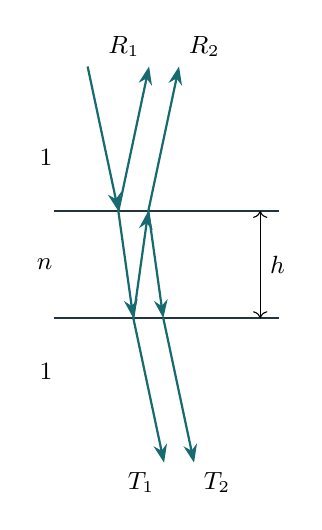
\begin{tikzpicture}[scale=.68]
\draw[object](-1.2,0)--(3,0) (-1.2,-2)--(3,-2);
\node[left]at(-1.05,1){$1$};\node[left]at(-1.05,-1){$n$};\node[left]at(-1.05,-3){$1$};
\draw[motion](-0.57390272,2.70000000)--(0,0);
\draw[motion](0,0)--(0.57390272,2.70000000);
\draw[motion](0,0)--(0.27991753,-2.00000000);
\draw[motion](0.27991753,-2.00000000)--(0.55983507,0.00000000);
\draw[motion](0.55983507,0.00000000)--(1.13373778,2.70000000);
\draw[motion](0.27991753,-2.00000000)--(0.85382025,-4.70000000);
\draw[motion](0.55983507,0.00000000)--(0.83975260,-2.00000000);
\draw[motion](0.83975260,-2.00000000)--(1.41365532,-4.70000000);
\node[above left]at(0.57390272,2.70000000){$R_1$};
\node[above right]at(1.13373778,2.70000000){$R_2$};
\node[below left]at(0.85382025,-4.70000000){$T_1$};
\node[below right]at(1.41365532,-4.70000000){$T_2$};
\draw[<->](2.65,0)--(2.65,-2);\node[right]at(2.65,-1){$h$};

\end{tikzpicture}
\figcaption{图光2.23\quad 两束截断光路；图取$\theta_0=12^\circ$满足折射定律，数值取正入射极限}
\end{minipage}\end{center}

\workarea

\clearpage

\pdfbookmark[2]{第 24 题 单层减反膜的厚度与波长响应}{q24}

\section*{第 24 题\quad 单层减反膜的厚度与波长响应}\label{q:24}

折射率$n_g=1.50$的玻璃表面镀一层$n_f=1.38$的氟化镁，空气折射率为1。光从空气垂直入射，忽略材料色散、吸收和玻璃背面反射。（1）为使$\lambda_0=550\,\mathrm{nm}$反射最弱，求最小膜厚与反射率，并与未镀膜比较。（2）同一膜厚下，求$400\,\mathrm{nm}$与$700\,\mathrm{nm}$的反射率。分别用双光束近似与完整多光束式给出反射率。

\begin{center}\begin{minipage}{.98\linewidth}\centering
\begin{tikzpicture}[scale=.86,transform shape]
\draw[object] (-1.3,0)--(5.5,0);\draw[object] (-1.3,-1.2)--(5.5,-1.2);
\node[left] at (-1.3,.7) {$n_0=1$};\node[left] at (-1.3,-.6) {$n_f=1.38$};\node[left] at (-1.3,-1.65) {$n_g=1.50$};
% ray:Q-direct
\draw[<->,thick,color=accent] (0,0)--(0,1.7);
\node[left] at (0,1.2) {$E_0\downarrow$};\node[right] at (0,1.2) {$R_1\uparrow$};
% ray:Q-bottom
\draw[<->,thick,color=warm] (2.5,-1.2)--(2.5,0);
\draw[motion] (2.5,0)--(2.5,1.7);
\node[right] at (2.5,1.15) {$R_2$};
\draw[guide] (-.6,1.7)--(3.5,1.7);
\node[above] at (1.4,1.7) {同一参考面};
\draw[<->,thin] (4.6,-1.2)--(4.6,0);\node[right] at (4.6,-.6) {$t$};
\node[below] at (1.5,-1.8) {两列分示两种贡献，各段均沿法线};
\end{tikzpicture}
\figcaption{图光2.24\quad 正入射薄膜反射路径的分列表示}
\end{minipage}\end{center}

\workarea

\clearpage

\pdfbookmark[2]{第 25 题 半球发光器件的增透设计}{q25}

\section*{第 25 题\quad 半球发光器件的增透设计}\label{q:25}

砷化镓发光器件做成半球，发光区位于球心；发光波长$\lambda=930\,\mathrm{nm}$，砷化镓折射率$n_1=3.4$，外部空气$n_2=1$。忽略吸收与色散，膜厚远小于球半径。（1）求未镀膜时球面的反射率。（2）求使反射完全消失的单层膜折射率与最小厚度。（3）分别用$n=1.38$氟化镁、$n=2.38$硫化锌，并各取自身设计四分之一波厚度，求反射率，判断能否增透。
\begin{center}\begin{minipage}{.98\linewidth}\centering
\begin{tikzpicture}[scale=.85]
\draw[object](-3,0)--(3,0);
\draw[object](2.6,0)arc[start angle=0,end angle=180,radius=2.6];
\draw[object](2.8,0)arc[start angle=0,end angle=180,radius=2.8];
\fill(0,0)circle(.035);\node[below]at(0,0){$O$};
\node at(1.1,1.5){$n_1=3.4$};
\node[left]at(-3,2.3){空气$n_2=1$};
\draw[guide](1.97989899,1.97989899)--(3.2,2.1);
\node[right]at(3.2,2.1){膜$n,t$};
\draw[motion](0,0)--(2.35640025,1.09880748);
\draw[motion](2.35640025,1.09880748)--(2.53766180,1.18333113);
\draw[motion](2.53766180,1.18333113)--(2.99081570,1.39464026);
\draw[motion](0,0)--(0.00000000,2.60000000);
\draw[motion](0.00000000,2.60000000)--(0.00000000,2.80000000);
\draw[motion](0.00000000,2.80000000)--(0.00000000,3.30000000);
\draw[motion](0,0)--(-2.35640025,1.09880748);
\draw[motion](-2.35640025,1.09880748)--(-2.53766180,1.18333113);
\draw[motion](-2.53766180,1.18333113)--(-2.99081570,1.39464026);

\end{tikzpicture}
\figcaption{图光2.25\quad 球心发光区的三条径向光线均正入射；膜厚示意放大}
\end{minipage}\end{center}

\workarea

\clearpage

\pdfbookmark[2]{第 26 题 单层多光束求和与双层减反}{q26}

\section*{第 26 题\quad 单层多光束求和与双层减反}\label{q:26}

折射率$n$、厚度$h$的无损薄膜夹在入射介质$n_0$与基底$n_G$之间，单色光正入射。（1）从各次反射电场的级数求和，推导完整强度反射率，并写成$\cos^2(\delta/2)$、$\sin^2(\delta/2)$形式，$\delta=4\pi nh/\lambda$。（2）求单层完全减反条件。（3）在基底上先镀$n_H$高折射率层，再镀$n_L$低折射率层，每层光学厚度$\lambda/4$，求完全减反的匹配条件。

\begin{center}\begin{minipage}{.98\linewidth}\centering
\begin{tikzpicture}[scale=.86,transform shape]
\draw[object] (-3,0)--(0,0);\draw[object] (-3,-1.2)--(0,-1.2);
\node[left] at (-3,.5) {$n_0$};\node[left] at (-3,-.6) {$n$};\node[left] at (-3,-1.6) {$n_G$};
% ray:Q-single
\draw[motion] (-1.5,1.4)--(-1.5,0);
\draw[<->] (-.4,-1.2)--(-.4,0);\node[right] at (-.4,-.6) {$h$};
\draw[object] (2,0)--(6,0);\draw[object] (2,-.9)--(6,-.9);\draw[object] (2,-1.8)--(6,-1.8);
\node[left] at (2,.5) {$n_0$};\node[left] at (2,-.45) {$n_L$};\node[left] at (2,-1.35) {$n_H$};\node[left] at (2,-2.1) {$n_G$};
% ray:Q-double
\draw[motion] (4,1.4)--(4,0);
\node[right] at (6,-.45) {$n_Lh_L=\lambda/4$};
\node[right] at (6,-1.35) {$n_Hh_H=\lambda/4$};
\node[below] at (-1.4,-2.4) {单层：正入射};
\node[below] at (4.4,-2.4) {双层：从外侧先低后高};
\end{tikzpicture}
\figcaption{图光2.26\quad 单层及双层膜的介质次序，层厚作符号示意}
\end{minipage}\end{center}

\workarea

\clearpage

\pdfbookmark[2]{第 27 题 交替四分之一波层的高反射膜}{q27}

\section*{第 27 题\quad 交替四分之一波层的高反射膜}\label{q:27}

玻璃基底$n_G$上镀交替的高、低折射率无损薄膜，折射率为$n_H>n_L$，每层光学厚度均为设计波长的$\lambda/4$。从空气侧依次为$H,L,H,\ldots,L,H$，共$2k+1$层，基底侧和外侧均邻接高折射率层。外界折射率$n_0$。（1）推导正入射设计波长的强度反射率。（2）$n_0=1,n_G=1.50,n_H=2.40,n_L=1.38$时，求五层与九层膜的反射率，并说明增加层数的适用范围。

\begin{center}\begin{minipage}{.98\linewidth}\centering
\begin{tikzpicture}[every node/.style={font=\small},x=1.55cm,y=1.1cm]
\draw[object,fill=accent!6](0.000000000000,-0.5)rectangle(0.613854166667,1.2);\node at(0.306927083333,0.350000000000){$H$};
\draw[object,fill=warm!6](0.613854166667,-0.5)rectangle(1.681426630435,1.2);\node at(1.147640398551,0.350000000000){$L$};
\draw[object,fill=accent!6](1.681426630435,-0.5)rectangle(2.295280797101,1.2);\node at(1.988353713768,0.350000000000){$H$};
\draw[object,fill=warm!6](2.295280797101,-0.5)rectangle(3.362853260870,1.2);\node at(2.829067028986,0.350000000000){$L$};
\draw[object,fill=accent!6](3.362853260870,-0.5)rectangle(3.976707427536,1.2);\node at(3.669780344203,0.350000000000){$H$};
% SERIES normal_path
\draw[guide] plot coordinates {(-1.000000000000,0.000000000000) (4.976707427536,0.000000000000)};
\draw[motion](-.95,0)--(-.30,0);\draw[motion](4.126707427536,0)--(4.826707427536,0);
\node[left]at(-.15,.9){$n_0$};\node[right]at(4.126707427536,.9){$n_G$};\draw[<->,muted](0,-.85)--(0.613854166667,-.85) node[midway,below]{$h_H$};\draw[<->,muted](0.613854166667,-.85)--(1.681426630435,-.85) node[midway,below]{$h_L$};\node[above]at(1.988353713768,1.5){$n_Hh_H=n_Lh_L=\lambda_0/4$};\node[below]at(1.988353713768,-1.35){法线方向$z$；层宽单位为$100\,\mathrm{nm}$};
\end{tikzpicture}
\figcaption{图光2.27\quad 五层示意：两端均为高折射率层；层宽按实际厚度比例}
\end{minipage}\end{center}

\workarea

\end{document}
